\documentclass[pdflatex,compress]{beamer}

%\usetheme[dark,framenumber,totalframenumber]{ElektroITK}
\usetheme[darktitle,framenumber,totalframenumber]{ElektroITK}

\usepackage{graphicx}

\title{PEMODELAN JARINGAN KOMUNIKASI}
\subtitle{Subnetting}

\author{Mifta Nur Farid, S.T., M.T.}

\begin{document}

\maketitle

\section{CIDR Classless Inter-Domain Routing}

\begin{frame}
	\frametitle{CIDR Classless\\Inter-Domain Routing}
	\begin{itemize}
		\item A problem with classful addresses was that if a company had more than 254 hosts they would need to be assigned a Class B network
		\item They would have much less than the 65,534 hosts allocated, so this wasted a huge amount of the global address space
		\item Classless Inter-Domain Routing (CIDR) was introduced in 1993 to alleviate this problem
	\end{itemize}
\end{frame}

\begin{frame}
	\frametitle{CIDR Classless\\Inter-Domain Routing}
	\begin{itemize}
		\item CIDR removed the fixed /8, /16 and /24 requirements for the address classes, and allowed them to be split or 'subnetted' into smaller networks
		\item For example 175.10.10.0/20
		\item Companies can now be allocated an address range which more closely matches their needs and does not waste addresses
	\end{itemize}
\end{frame}

\begin{frame}
	\frametitle{CIDR and Route Summarisation}
	\begin{itemize}
		\item Another benefit of CIDR is that aggregate blocks of networks can be advertised on the Internet
	\end{itemize}
	\begin{center}
		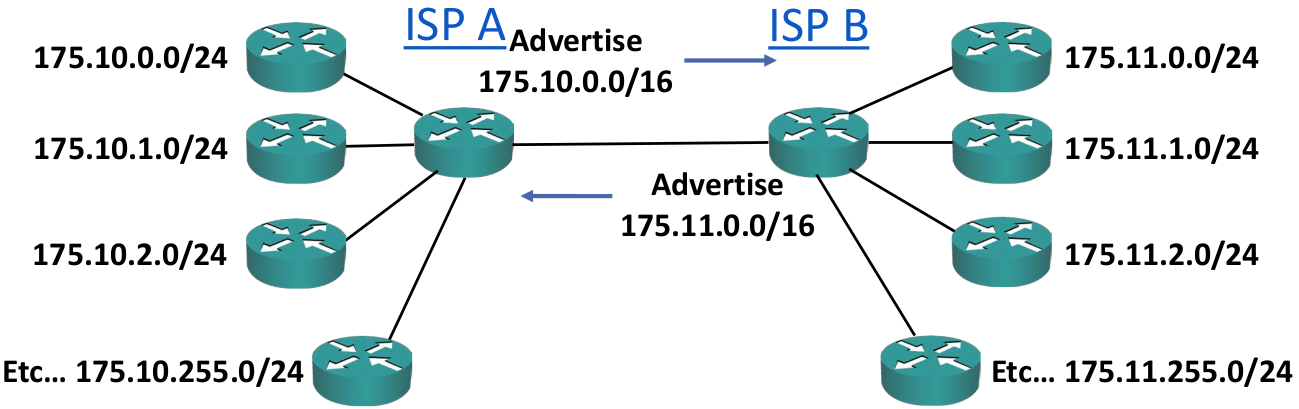
\includegraphics[width=1\linewidth]{img/img01}
	\end{center}
\end{frame}

\begin{frame}
	\frametitle{Route Summarisation Benefits}
	\begin{itemize}
		\item ISP A does not know about all 256 /24 networks reachable in ISP B
		\item It only has the single 175.11.0.0/16 summary route
		\item This reduces the size of ISP A’s routing table and takes up less memory
		\item If an individual link goes down in ISP B, it has no impact on ISP A. The single summary route does not change
		\item (Routers in ISP B would have to recalculate their routing table if a link went down)
		\item This restricts issues to the local part of the network and reduces CPU load
	\end{itemize}
\end{frame}

\section{Subnetting Overview}

\begin{frame}
	\frametitle{Subnetting}
	\begin{itemize}
		\item To understand this lecture, think about it from the point of view of the originally intended IPv4 design again, where all hosts which can communicate on the Internet have a public IP address.
		\item Let’s say we’re the network designer for a small business with four departments spread over two offices, and we want to manage our own public address space.
		\item Rather than purchasing separate address ranges for the different departments, we can purchase a single range and subnet it into smaller portions.
	\end{itemize}
\end{frame}

\begin{frame}
	\frametitle{Borrowing Host Bits}
	\begin{itemize}
		\item Let's say we've been allocated Class C 200.15.10.0/24
	\end{itemize}

	\begin{center}
			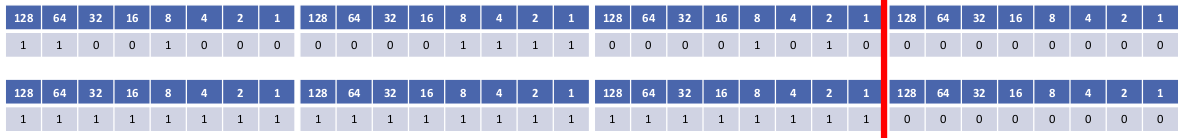
\includegraphics[width=1\linewidth]{img/img02}
	\end{center}

	\begin{itemize}
		\item To subnet the network into smaller subnets, we need to 'borrow' host bits and add them to the network portion of the address
		\item The network address line always moves to the right when we subnet
		\item The further to the right we go, the more subnets we'll have of that size but less hosts
	\end{itemize}
\end{frame}

\begin{frame}
	\frametitle{Calculating the Number of Networks}
	\begin{itemize}
		\item To calculate the number of available subnets, the formula is $ 2^{\text{subnet-bits}} $
		\item If a Class C network uses a /28 subnet mask then we've borrowed 4 bits from the default of /24
		\item $ 2^4 = 16 $ available subnets
		\item If a Class B network uses a /28 subnet mask then we've borrowed 12 bits from the default of /16
		\item $ 2^{12} = 4096 $ available subnets
		\item Hosts on different subnets need to go via a router if they want to
		communicate with each other
	\end{itemize}
\end{frame}

\begin{frame}
	\frametitle{Calculating the Number of Hosts}
	\begin{itemize}
		\item To calculate the number of available hosts, the formula is $ 2^{\text{host-bits}} - 2 $
		\item We subtract 2 because the network address and broadcast address cannot be assigned to hosts
		\item If a Class C network uses a /28 subnet mask then we have 4 bits left for hosts
		\item $ 2^4 - 2 = 14 $
		\item If a Class B network uses a /28 subnet mask then we have 4 bits left for hosts
		\item $ 2^4 - 2 = 14 $
	\end{itemize}
\end{frame}

\begin{frame}
	\frametitle{A Quick Note on ip subnet-zero}
	\begin{itemize}
		\item Just like we have to subtract 2 to get the number of valid hosts, we used to have to subtract 2 to get the number of available networks also
		\item In the original Internet standards, it was not allowed to use network bits of all 0's or all 1's (just like we can't use all host bits of all 0's or all 1's)
		\item There wasn't really any practical need for this and it wasted address space
		\item The \textit{ip subnet-zero} command on a router overrides the limitation, and is enabled by default
	\end{itemize}
\end{frame}

\section{Subnetting Class C Networks and VLSM}

\begin{frame}
	\frametitle{Class C /31 Subnet}
	\begin{itemize}
		\item Let's say we've been allocated Class C 200.15.10.0/24
	\end{itemize}
	\begin{center}
		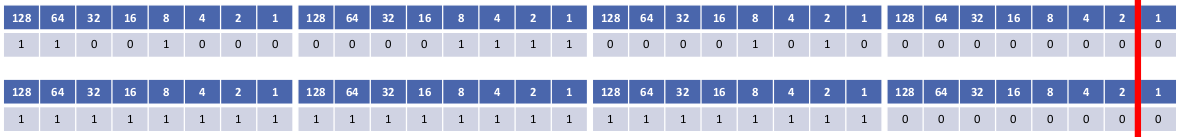
\includegraphics[width=1\linewidth]{img/img03}
	\end{center}
	\begin{itemize}
		\item If we move the line all the way to the right we're now using /31 (or 255.255.255.254)
		\item This leaves one bit for the host address, with a possible value of 0 or 1
		\item It borrows 7 bits for the network address
		\item This gives us 128 subnets ($ 2^7 $) which accommodate 2 hosts each
	\end{itemize}
\end{frame}

\begin{frame}
	\frametitle{Class C /31 Subnet}
	\begin{itemize}
		\item Let’s say we’ve been allocated Class C 200.15.10.0/24.
	\end{itemize}
	\begin{center}
		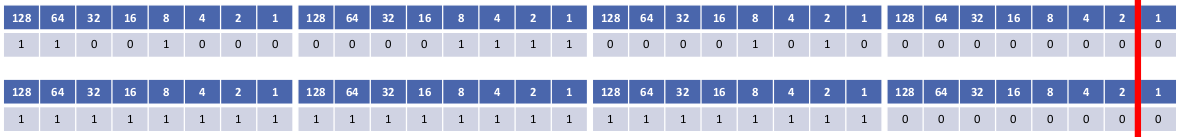
\includegraphics[width=1\linewidth]{img/img03}
	\end{center}
	\begin{itemize}
		\item If we move the line all the way to the right we're now using /31 (or 255.255.255.254)
		\item This leaves one bit for the host address, with a possible value of 0 or 1
		\item It borrows 7 bits for the network address
		\item This gives us 128 subnets ($ 2^7 $) which accommodate 2 hosts each
	\end{itemize}
\end{frame}

\end{document}